\subsection{Headers}

\begin{figure}
  \begin{center}
  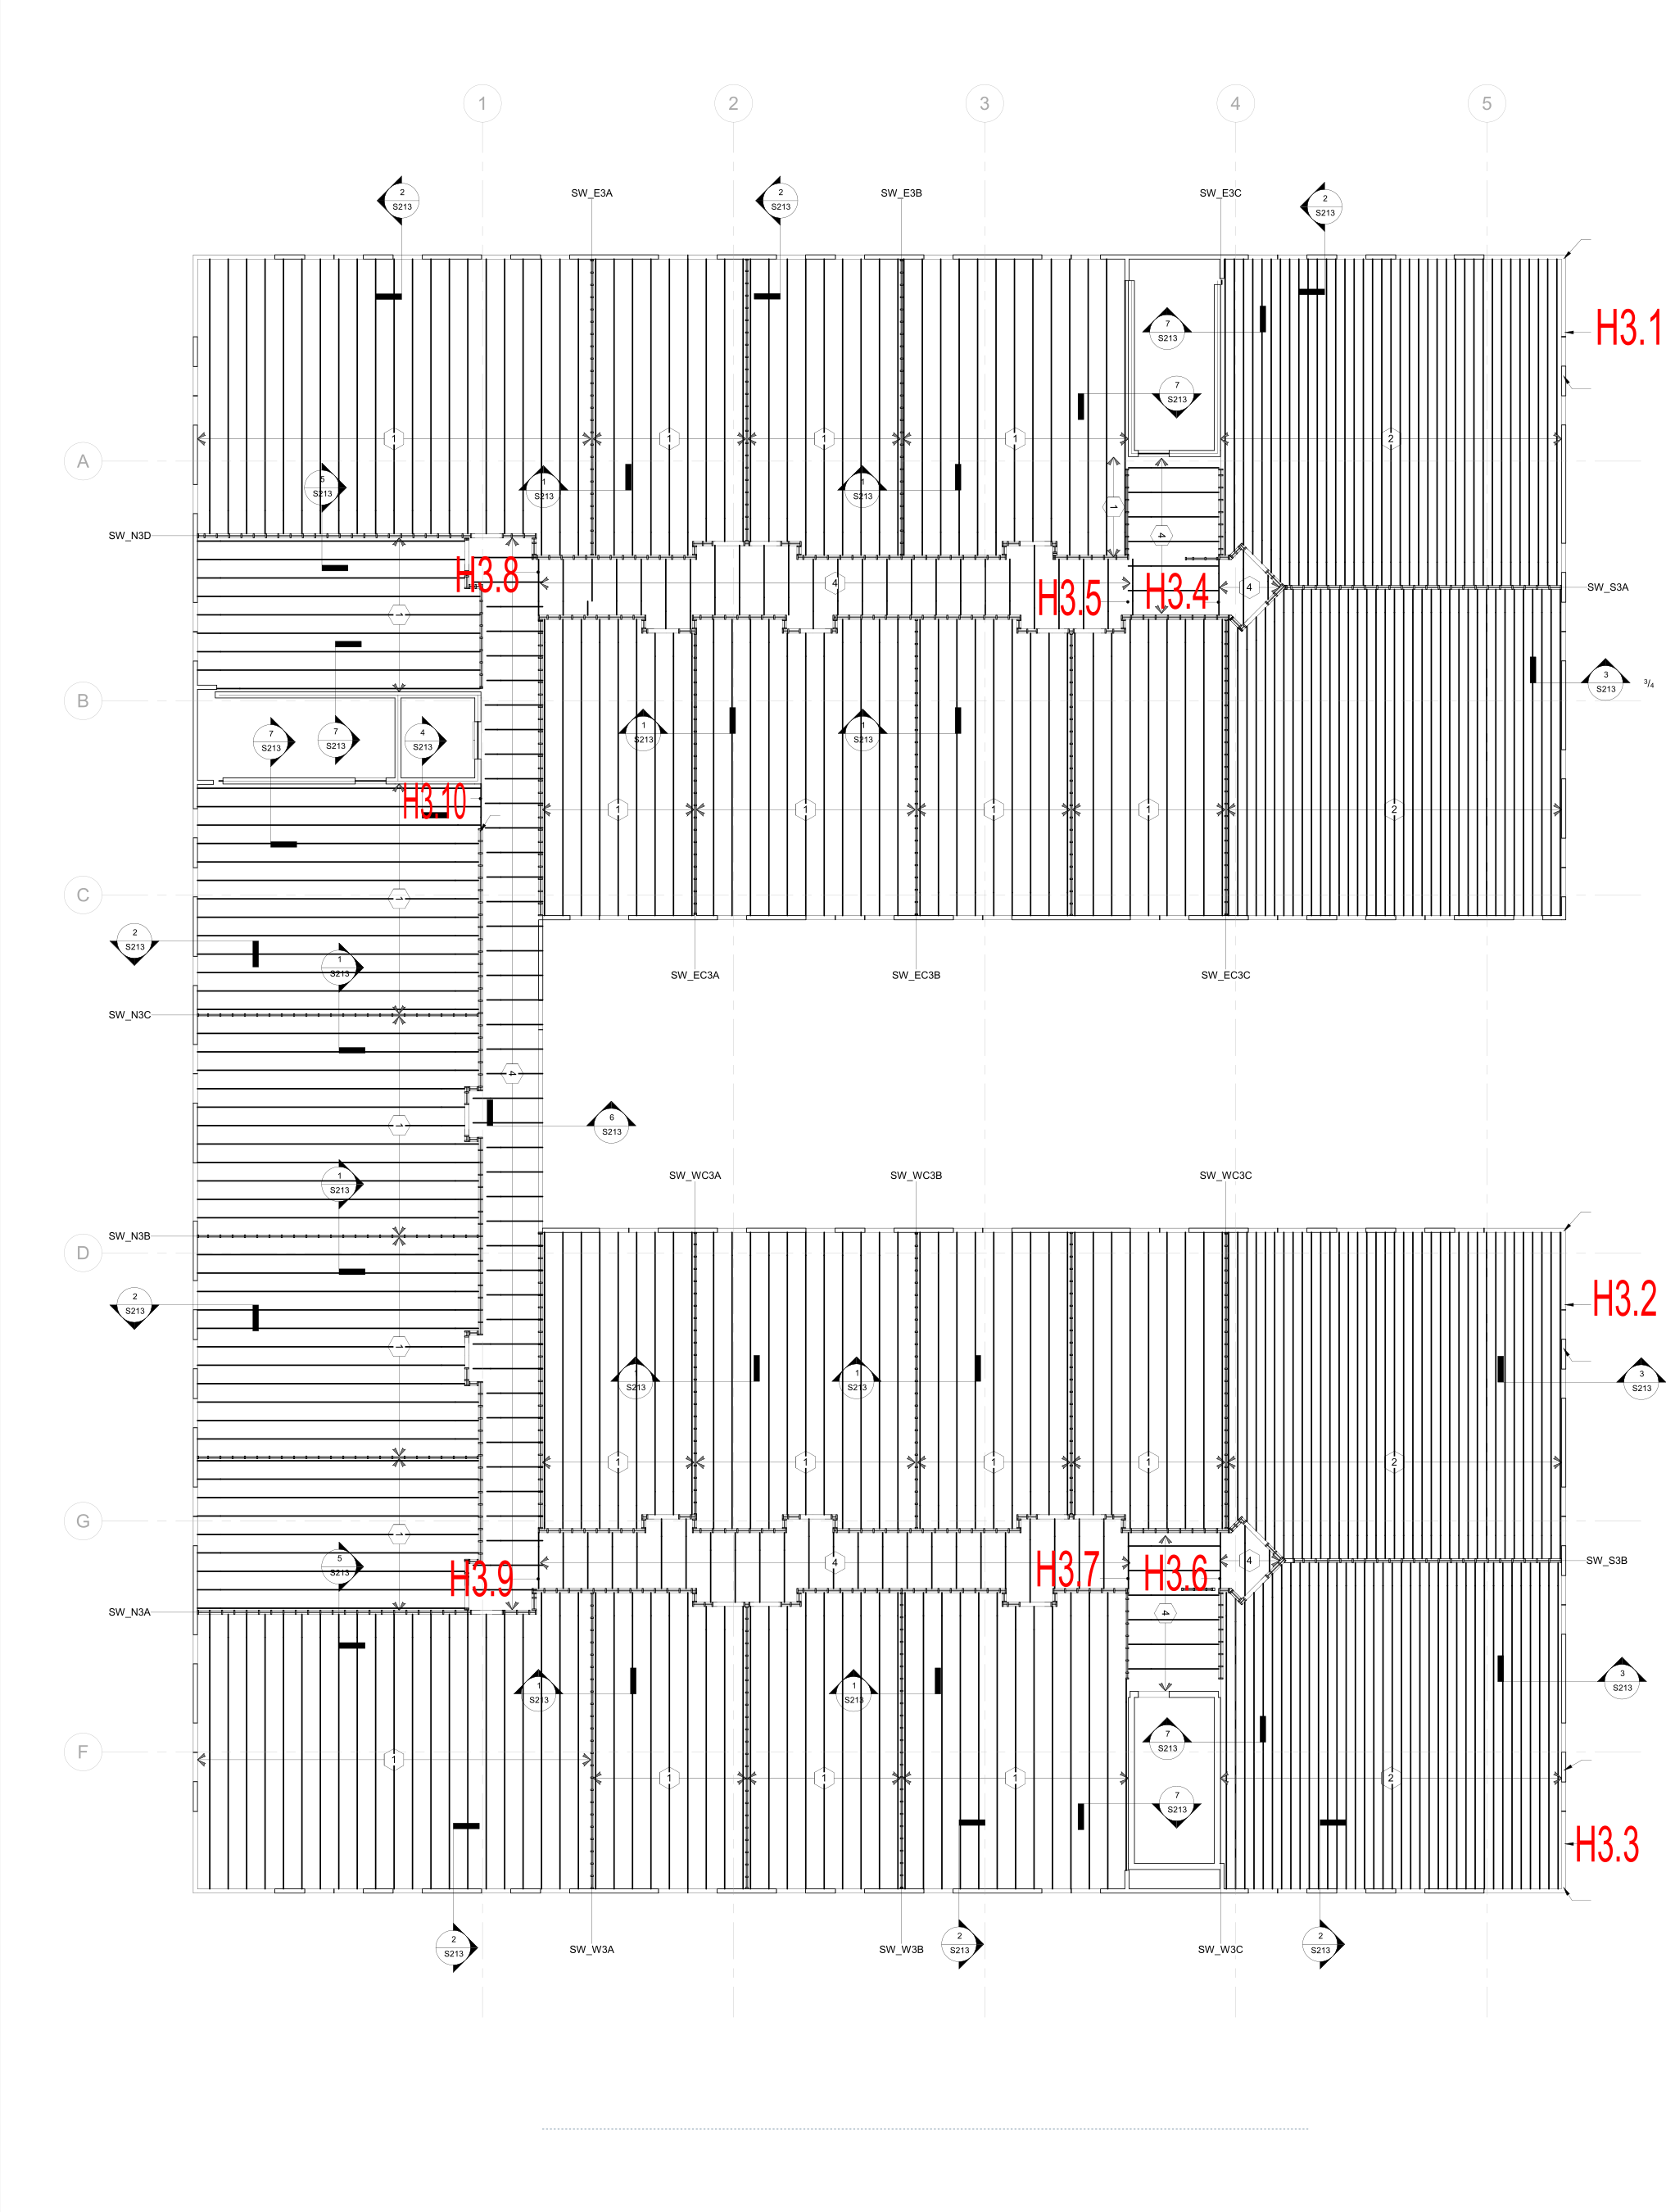
\includegraphics[width=120mm]{figures/headers_key_plan_roof}
  \end{center}
  \caption{Headers key plan. Roof}\label{fg_headers_key_plan_roof}
\end{figure}

\begin{figure}
  \begin{center}
  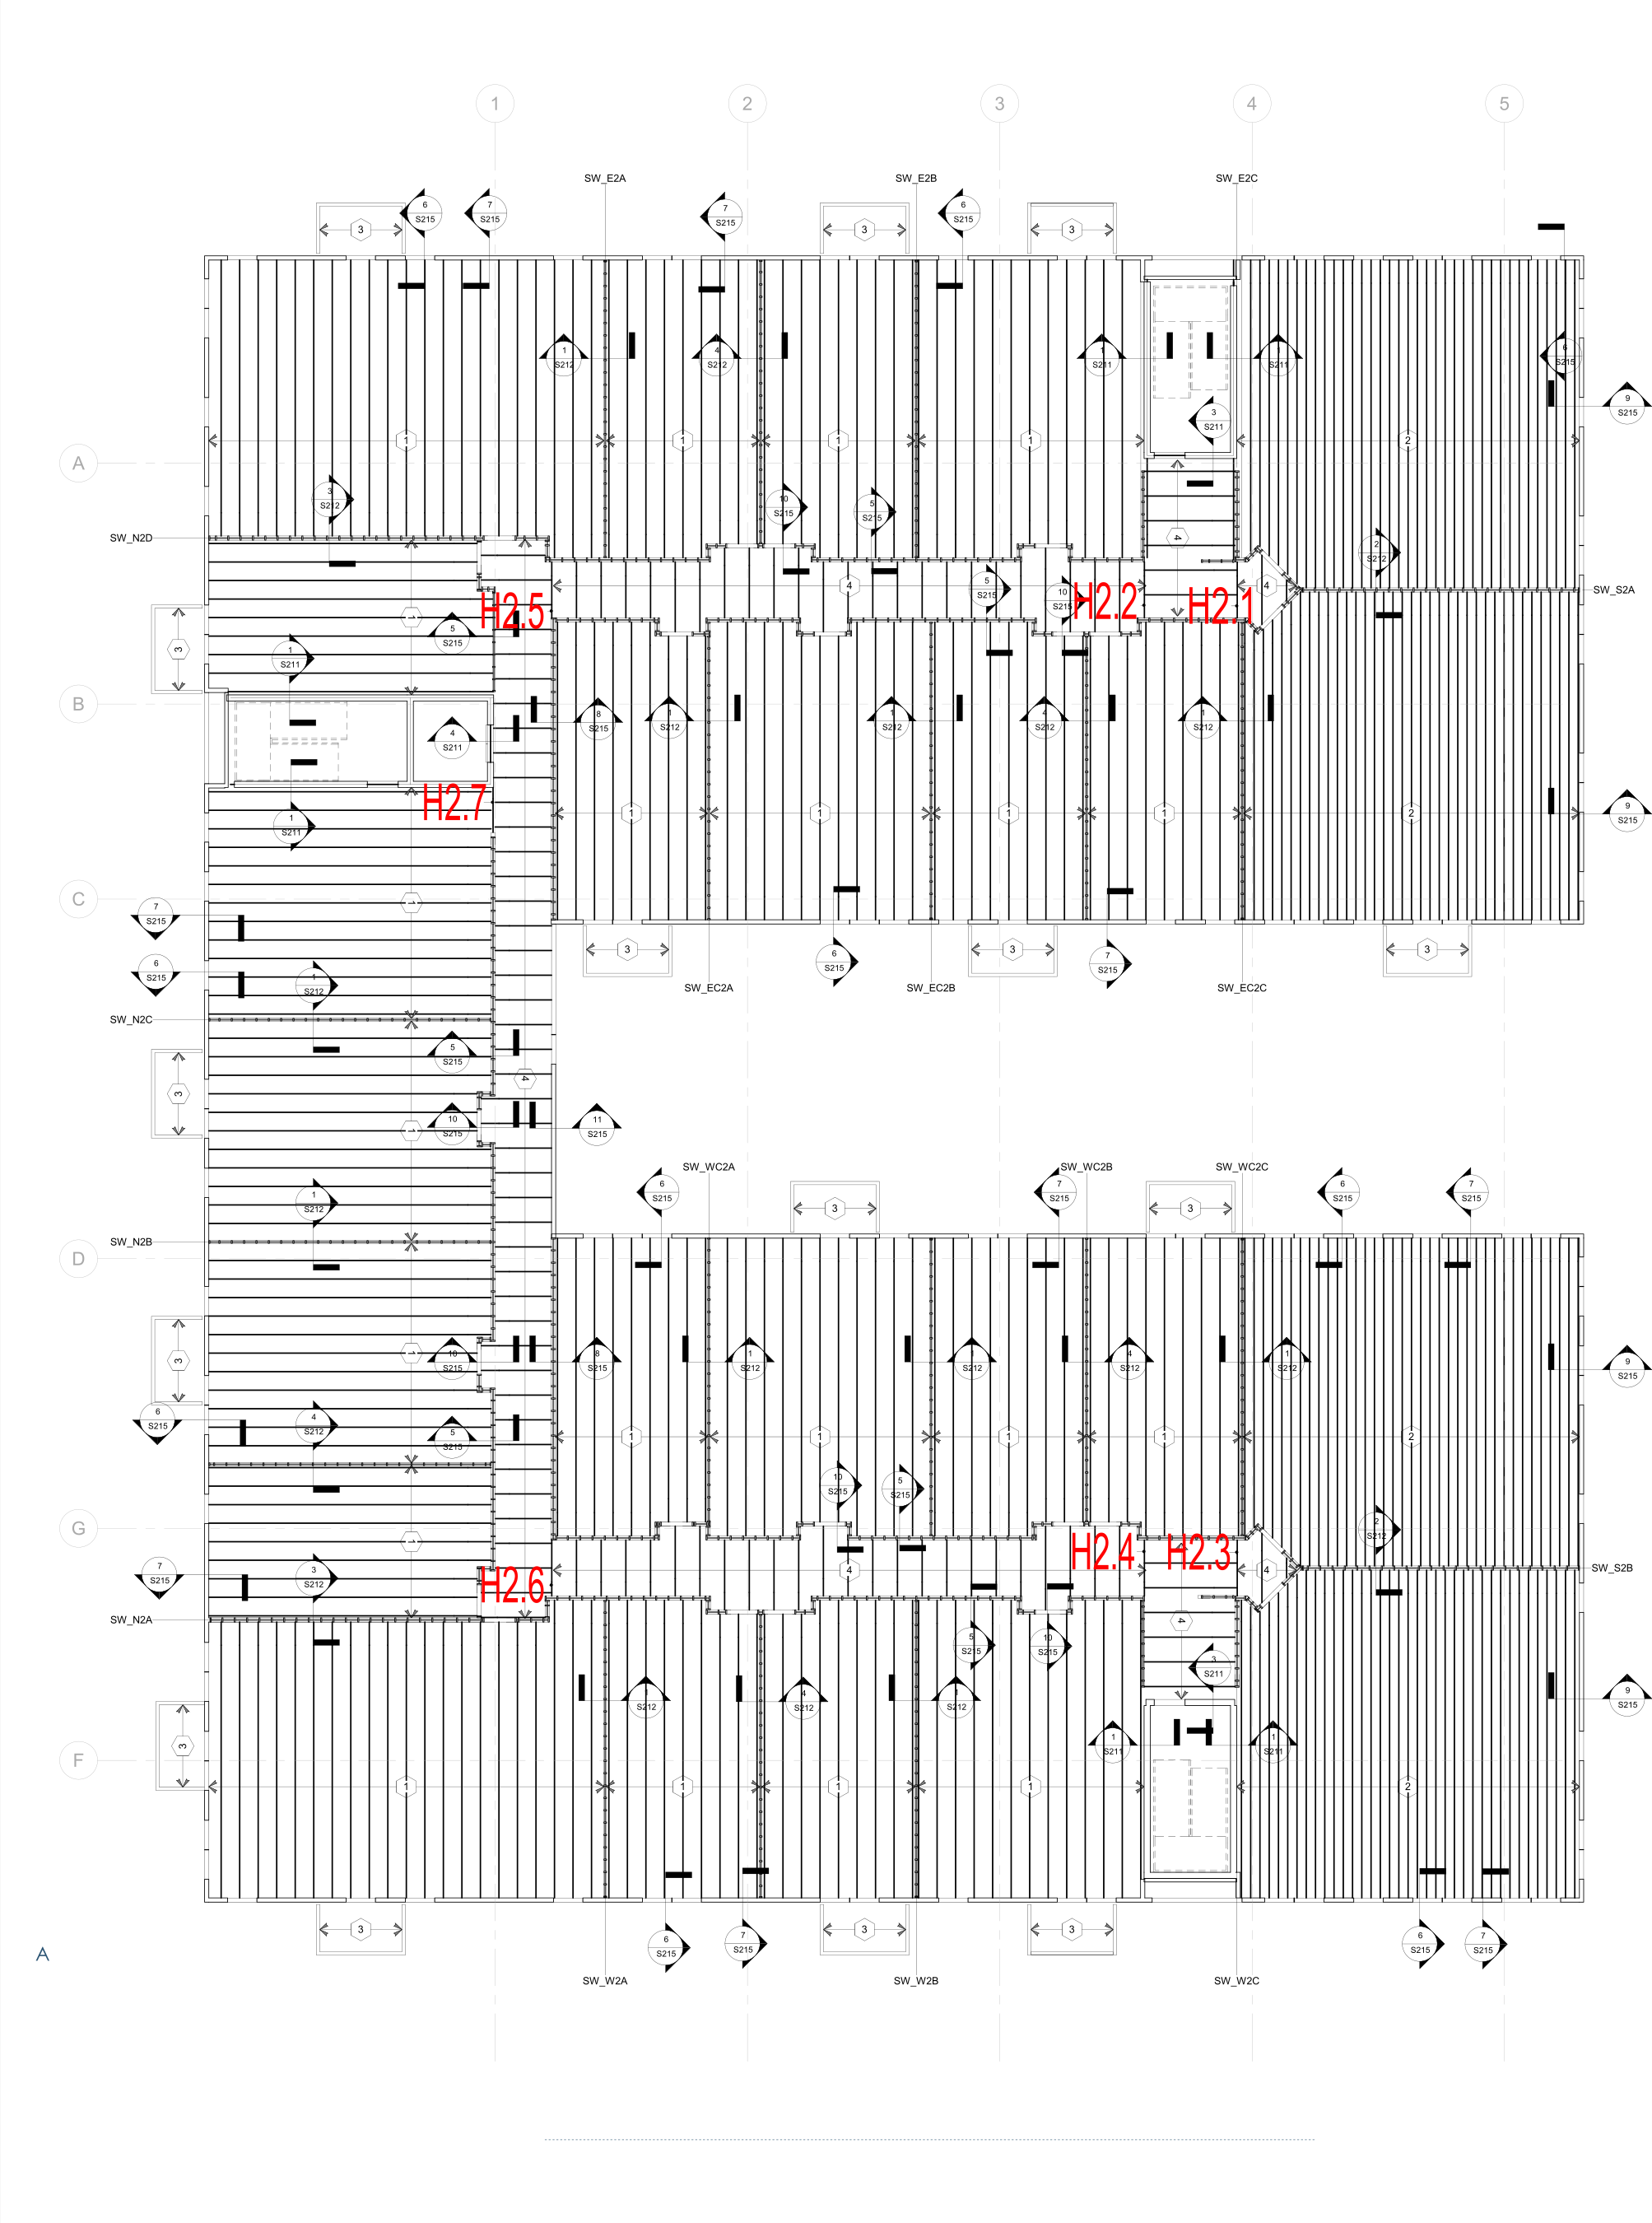
\includegraphics[width=120mm]{figures/headers_key_plan_3rd_floor}
  \end{center}
  \caption{Headers key plan. Third floor}\label{fg_headers_key_plan_3rd_floor}
\end{figure}

\begin{figure}
  \begin{center}
  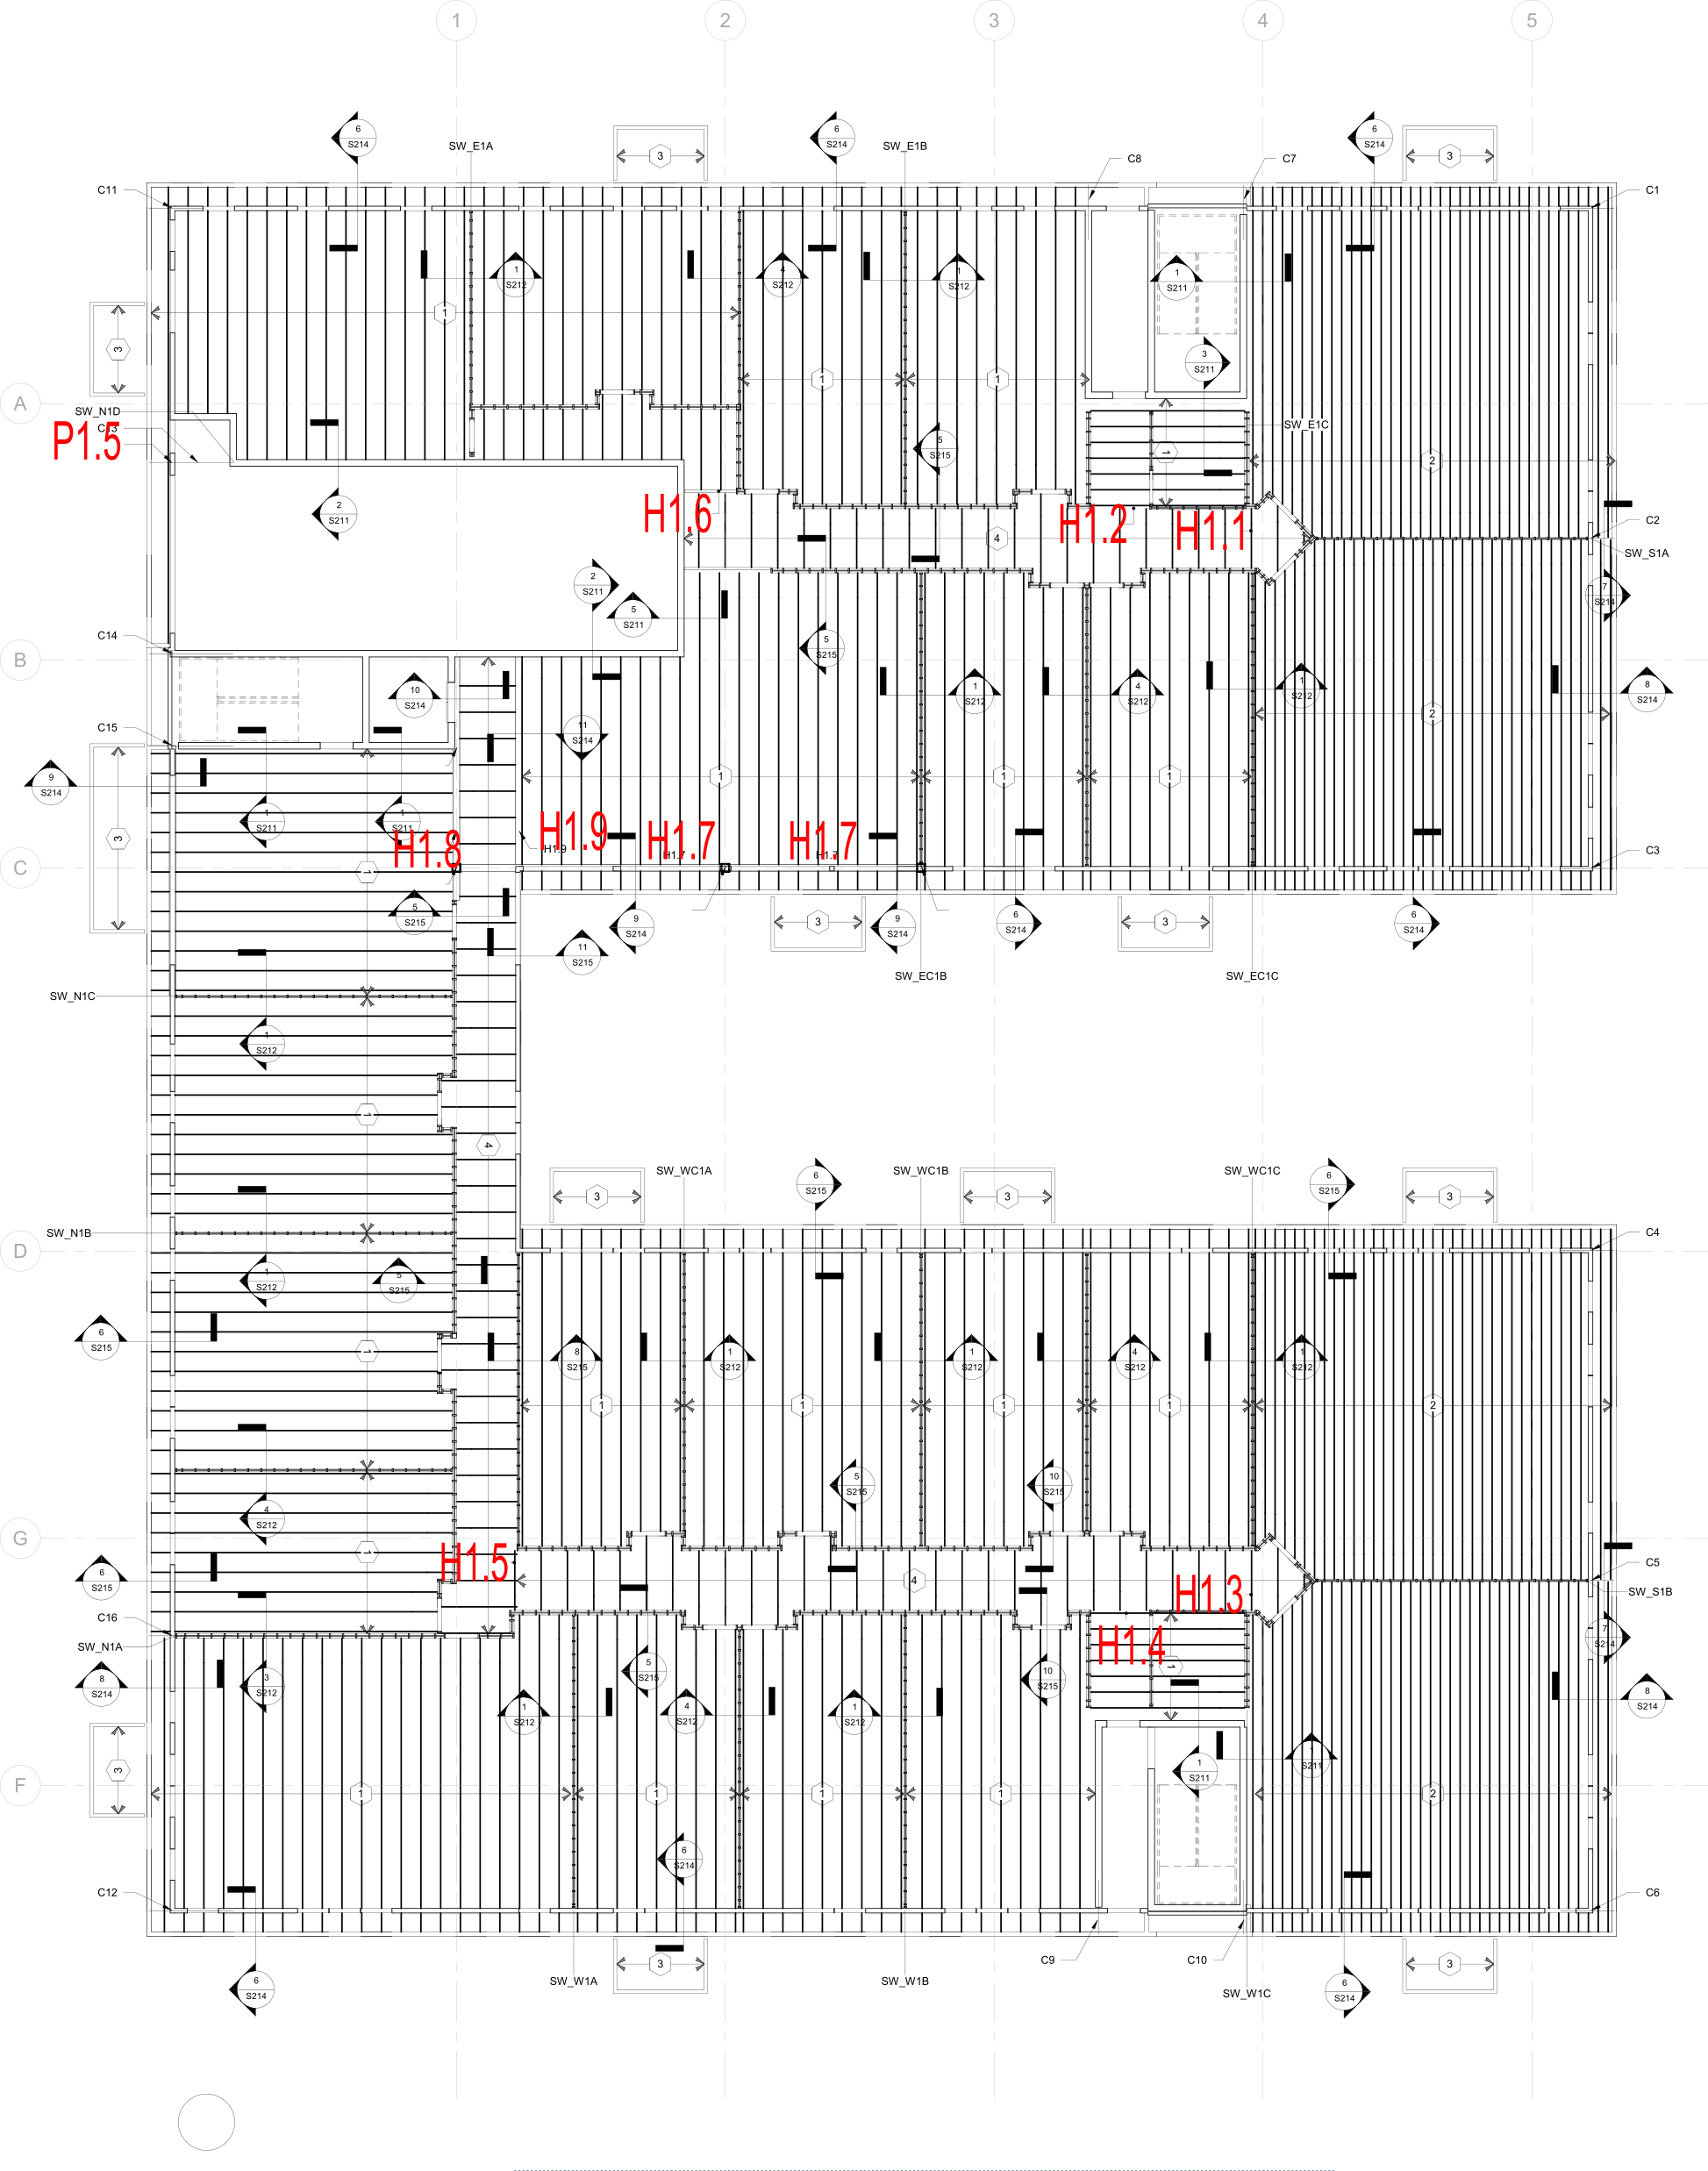
\includegraphics[width=120mm]{figures/headers_key_plan_2nd_floor}
  \end{center}
  \caption{Headers key plan. Second floor}\label{fg_headers_key_plan_2nd_floor}
\end{figure}

\subsubsection{Third floor enclosed balconies headers (H3.1 to H3.3)}
Simply supported 1.75x14 LSL 1.55E headers.

\paragraph{Structural design of the header.}

\subparagraph{Design load.}

\begin{equation}
  w_{load}= 1.75\ kN/m
\end{equation}

\subparagraph{Internal forces.}

\noindent Maximum induced moment:

\begin{equation}
  M_{max}= w_{load} \frac{L^2}{8}= 1.65\ kN m
\end{equation}

\noindent Maximum induced shear:

\begin{equation}
  V_{max}= w_{load} \frac{L}{2}= 2.40\ kN
\end{equation}

\subparagraph{Structural bending check.}

\noindent Design resisting moment:

\begin{equation}
  M'_s= 14.96\ kN m
\end{equation}

\noindent Structural bending check: $M'_s = 14.96 > 1.65 = M_{max} \implies OK$

\subparagraph{Structural shear check.}

\noindent Design resisting shear:
\begin{equation}
  V'_s= 29.79\ kN
\end{equation}

\noindent Structural shear check: $V'_s = 29.79 > 2.40 = V_{max} \implies OK$

\subparagraph{Bending stiffness.}
The deflection obtained is:

\begin{equation}
  \Delta_{TL}= 0.72\ mm= \frac{L}{3781} < \frac{L}{360} \implies OK
\end{equation}

\subsubsection{Corridor headers (H3.4 to H3.9, H2.1 to H2.6 and H1.1 to H1.6)}
Simply supported 3.5x7-1/4'' LVL headers.

\paragraph{Structural design of the header.}

\subparagraph{Design load.}

\begin{equation}
  w_{load}= 5.26\ kN/m
\end{equation}

\subparagraph{Internal forces.}

\noindent Maximum induced moment:

\begin{equation}
  M_{max}= w_{load} \frac{L^2}{8}= 2.29\ kN m
\end{equation}

\noindent Maximum induced shear:

\begin{equation}
  V_{max}= w_{load} \frac{L}{2}= 5.21\ kN
\end{equation}

\subparagraph{Structural bending check.}

\noindent Design resisting moment:

\begin{equation}
  M'_s= 10.63\ kN m
\end{equation}

\noindent Structural bending check: $M'_s = 10.63 > 2.29 = M_{max} \implies OK$

\subparagraph{Structural shear check.}

\noindent Design resisting shear:
\begin{equation}
  V'_s= 21.44\ kN
\end{equation}

\noindent Structural shear check: $V'_s = 21.44 > 5.21 = V_{max} \implies OK$

\subparagraph{Bending stiffness.}
The deflection obtained is:

\begin{equation}
  \Delta_{TL}= 0.07\ mm= \frac{L}{27939} < \frac{L}{360} \implies OK
\end{equation}

\paragraph{Fire design of the header.}
For the fire design of the header, mass loss due to charring is conservatively neglected, so the loading is unchanged. Therefore, the maximum induced moment and shear are unchanged. The fire resistance must be calculated.

\subparagraph{Mechanical properties of the burned section.}

\noindent Effective char depth:
\begin{equation}
  a_{eff}= 0.7 \times 10^{-3} \times 30 + 7 \times 10^{-3}= 28\ mm
\end{equation}

\noindent section modulus for a joist exposed on three sides:
\begin{equation}
  S_s= 133.70 \times 10^{-6}\ m^3
\end{equation}

\noindent shear area for a beam exposed on three sides:
\begin{equation}
  A_f= 51.37\ cm^2
\end{equation}

\noindent Adjusted allowable bending stress with $C_{fire}= 2.85$, $C_r= 1.0$, $C_D= 1.0$,$C_M= 1.0$, $C_t= 1.0$
\begin{equation}
  F'_{b,f}= 60.26\ MPa
\end{equation}

\noindent Adjusted allowable shear stress with  $C_{fire}= 2.85$, $C_D= 1.0$,$C_M= 1.0$, $C_t= 1.0$:
\begin{equation}
  F'_{v,f}= 5.40\ MPa
\end{equation}

\subparagraph{Structural bending check.}

\noindent Design resisting moment:

\begin{equation}
  M'_f= 8.06\ kN m
\end{equation}

\noindent Structural bending check: $M'_s = 8.06 > 2.29 = M_{max} \implies OK$

\subparagraph{Structural shear check.}

\noindent Design resisting shear:
\begin{equation}
  V'_f= 18.51\ kN
\end{equation}

\noindent Structural shear check: $V'_s = 18.51 > 5.21 = V_{max} \implies OK$

\subsubsection{Headers H3.10 and H2.7}
Simply supported 3.5x14'' LVL header.

\paragraph{Structural design of the header.}

\subparagraph{Design load.}

\begin{equation}
  w_{load}= 18.11\ kN/m
\end{equation}

\subparagraph{Internal forces.}

\noindent Maximum induced moment:

\begin{equation}
  M_{max}= w_{load} \frac{L^2}{8}= 10.94\ kN m
\end{equation}

\noindent Maximum induced shear:

\begin{equation}
  V_{max}= w_{load} \frac{L}{2}= 27.61\ kN
\end{equation}

\subparagraph{Structural bending check.}

\noindent Design resisting moment:

\begin{equation}
  M'_s= 36.65\ kN m
\end{equation}

\noindent Structural bending check: $M'_s = 36.65 > 10.94 = M_{max} \implies OK$

\subparagraph{Structural shear check.}

\noindent Design resisting shear:
\begin{equation}
  V'_s= 41.41\ kN
\end{equation}

\noindent Structural shear check: $V'_s = 41.41 > 27.61 = V_{max} \implies OK$

\subparagraph{Bending stiffness.}
The deflection obtained is:

\begin{equation}
  \Delta_{TL}= 0.33\ mm= \frac{L}{6027} < \frac{L}{360} \implies OK
\end{equation}

\paragraph{Fire design of the header.}
For the fire design of the header, mass loss due to charring is conservatively neglected, so the loading is unchanged. Therefore, the maximum induced moment and shear are unchanged. The fire resistance must be calculated.

\subparagraph{Mechanical properties of the burned section.}

\noindent Effective char depth:
\begin{equation}
  a_{eff}= 0.7 \times 10^{-3} \times 30 + 7 \times 10^{-3}= 28\ mm
\end{equation}

\noindent section modulus for a joist exposed on three sides:
\begin{equation}
  S_s= 588.48 \times 10^{-6}\ m^3
\end{equation}

\noindent shear area for a beam exposed on three sides:
\begin{equation}
  A_f= 107.78\ cm^2
\end{equation}

\noindent Adjusted allowable bending stress with $C_{fire}= 2.85$, $C_r= 1.0$, $C_D= 1.0$,$C_M= 1.0$, $C_t= 1.0$
\begin{equation}
  F'_{b,f}= 55.74\ MPa
\end{equation}

\noindent Adjusted allowable shear stress with  $C_{fire}= 2.85$, $C_D= 1.0$,$C_M= 1.0$, $C_t= 1.0$:
\begin{equation}
  F'_{v,f}= 5.40\ MPa
\end{equation}

\subparagraph{Structural bending check.}

\noindent Design resisting moment:

\begin{equation}
  M'_f= 32.8\ kN m
\end{equation}

\noindent Structural bending check: $M'_s = 32.80 > 10.93 = M_{max} \implies OK$

\subparagraph{Structural shear check.}

\noindent Design resisting shear:
\begin{equation}
  V'_f= 38.82\ kN
\end{equation}

\noindent Structural shear check: $V'_s = 38.82 > 27.605 = V_{max} \implies OK$

\subsubsection{Header H1.9}
Simply supported 5.25x18'' LVL 1.55E beam.

\paragraph{Structural design of the header.}

\subparagraph{Design load.}

\begin{equation}
  w_{load}= 4.77\ kN/m
\end{equation}

\subparagraph{Internal forces.}

\noindent Maximum induced moment:

\begin{equation}
  M_{max}= w_{load} \frac{L^2}{8}= 25.63\ kN m
\end{equation}

\noindent Maximum induced shear:

\begin{equation}
  V_{max}= w_{load} \frac{L}{2}= 15.73\ kN
\end{equation}

\subparagraph{Structural bending check.}

\noindent Design resisting moment:

\begin{equation}
  M'_s= 87.66\ kN m
\end{equation}

\noindent Structural bending check: $M'_s = 87.66 > 25.63 = M_{max} \implies OK$

\subparagraph{Structural shear check.}

\noindent Design resisting shear:
\begin{equation}
  V'_s= 79.87\ kN
\end{equation}

\noindent Structural shear check: $V'_s = 79.87 > 15.73 = V_{max} \implies OK$

\subparagraph{Bending stiffness.}
The deflection obtained is:

\begin{equation}
  \Delta_{TL}= 8.97\ mm= \frac{L}{735} < \frac{L}{600} \implies OK
\end{equation}


\subsubsection{Facade headers}
Simply supported 3.5x11 7/8 LSL 1.55E header.

\paragraph{Structural design of the header.}

\subparagraph{Design load.}

\begin{equation}
  w_{load}= 75.91\ kN/m
\end{equation}

\subparagraph{Internal forces.}

\noindent Maximum induced moment:

\begin{equation}
  M_{max}= w_{load} \frac{L^2}{8}= 8.26\ kN m
\end{equation}

\noindent Maximum induced shear:

\begin{equation}
  V_{max}= w_{load} \frac{L}{2}= 43.38\ kN
\end{equation}

\subparagraph{Structural bending check.}

\noindent Design resisting moment:

\begin{equation}
  M'_s= 21.96\ kN m
\end{equation}

\noindent Structural bending check: $M'_s = 21.96 > 8.26 = M_{max} \implies OK$

\subparagraph{Structural shear check.}

\noindent Design resisting shear:
\begin{equation}
  V'_s= 50.53\ kN
\end{equation}

\noindent Structural shear check: $V'_s = 50.53 > 43.38 = V_{max} \implies OK$

\subparagraph{Bending stiffness.}
The deflection obtained is:

\begin{equation}
  \Delta_{TL}= 0.41\ mm= \frac{L}{2758} < \frac{L}{600} \implies OK
\end{equation}

\subsubsection{Corridor headers}
Simply supported 3.5x16 LSL 1.55E header.

\paragraph{Structural design of the header.}

\subparagraph{Design load.}

\begin{equation}
  w_{load}= 118.11\ kN/m
\end{equation}

\subparagraph{Internal forces.}

\noindent Maximum induced moment:

\begin{equation}
  M_{max}= w_{load} \frac{L^2}{8}= 14.63\ kN m
\end{equation}

\noindent Maximum induced shear:

\begin{equation}
  V_{max}= w_{load} \frac{L}{2}= 72.0\ kN
\end{equation}

\subparagraph{Structural bending check.}

\noindent Design resisting moment:

\begin{equation}
  M'_s= 48.00\ kN m
\end{equation}

\noindent Structural bending check: $M'_s = 48.00 > 14.63 = M_{max} \implies OK$

\subparagraph{Structural shear check.}

\noindent Design resisting shear:
\begin{equation}
  V'_s= 76.60\ kN
\end{equation}

\noindent Structural shear check: $V'_s = 76.60 > 72.0 = V_{max} \implies OK$

\subparagraph{Bending stiffness.}
The deflection obtained is:

\begin{equation}
  \Delta_{TL}= 0.26\ mm= \frac{L}{4581} < \frac{L}{600} \implies OK
\end{equation}


